\section{Auswertung}
\label{sec:Auswertung}
\subsection{Überprüfung der Braggbedingung}
Zur Überprüfung der Braggbedingung wurde der Kristallwinkel auf $\SI{14}{\degree}$ eingestellt.
Die Messdaten befinden sich in Tabelle \ref{tab:bragg}.

\begin{table}
  \centering
  \caption{Messwerte zur Überprüfung der Braggbedingung.}
  \label{tab:bragg}
  \begin{tabular}[t]{c@{} S[table-format=2.1] S[table-format=3.0]}
   \toprule
     {$2\, \theta \, / \, \si{\degree}\:\:$} & {$\text{Rate} \, /  \, \si{\per\second}$} \\\midrule
     \csvreader[no head,
     late after line=\\,
     late after last line=\\\bottomrule,
     filter test={\ifnumless{\thecsvinputline}{22}}]%
     {data/braggbedingung.csv}{}%
     {$\SI{\csvcoli}{}$ & $\SI{\csvcolii}{}$}%
   \end{tabular}
   \begin{tabular}[t]{c@{} S[table-format=2.1] S[table-format=3.0]}
    \toprule
      {$2\, \theta \, / \, \si{\degree}\:\:$} & {$\text{Rate} \, /  \, \si{\per\second}$} \\\midrule
     \csvreader[filter test={\ifnumgreater{\thecsvinputline}{21}},
     late after line=\\,
     late after last line=\\\bottomrule]%
     {data/braggbedingung.csv}{}%
    {$\SI{\csvcoli}{}$ & $\SI{\csvcolii}{}$}%
  \end{tabular}
\end{table}
\begin{figure}
  \centering
  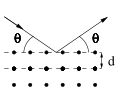
\includegraphics{bragg.pdf}
  \caption{Plot zur Überprüfung der Bragg-Bedingung.}
  \label{fig:bragg}
\end{figure}
Das Maximum der Intensität lässt sich aus dem Plot zu $\SI{13.9}{\degree}$ bestimmen und weicht um $\SI{0.7}{\percent}$ vom eingestellten Winkel ab.
